	\chapter{Piadas de Orientados e Orientadores}

\begin{center}
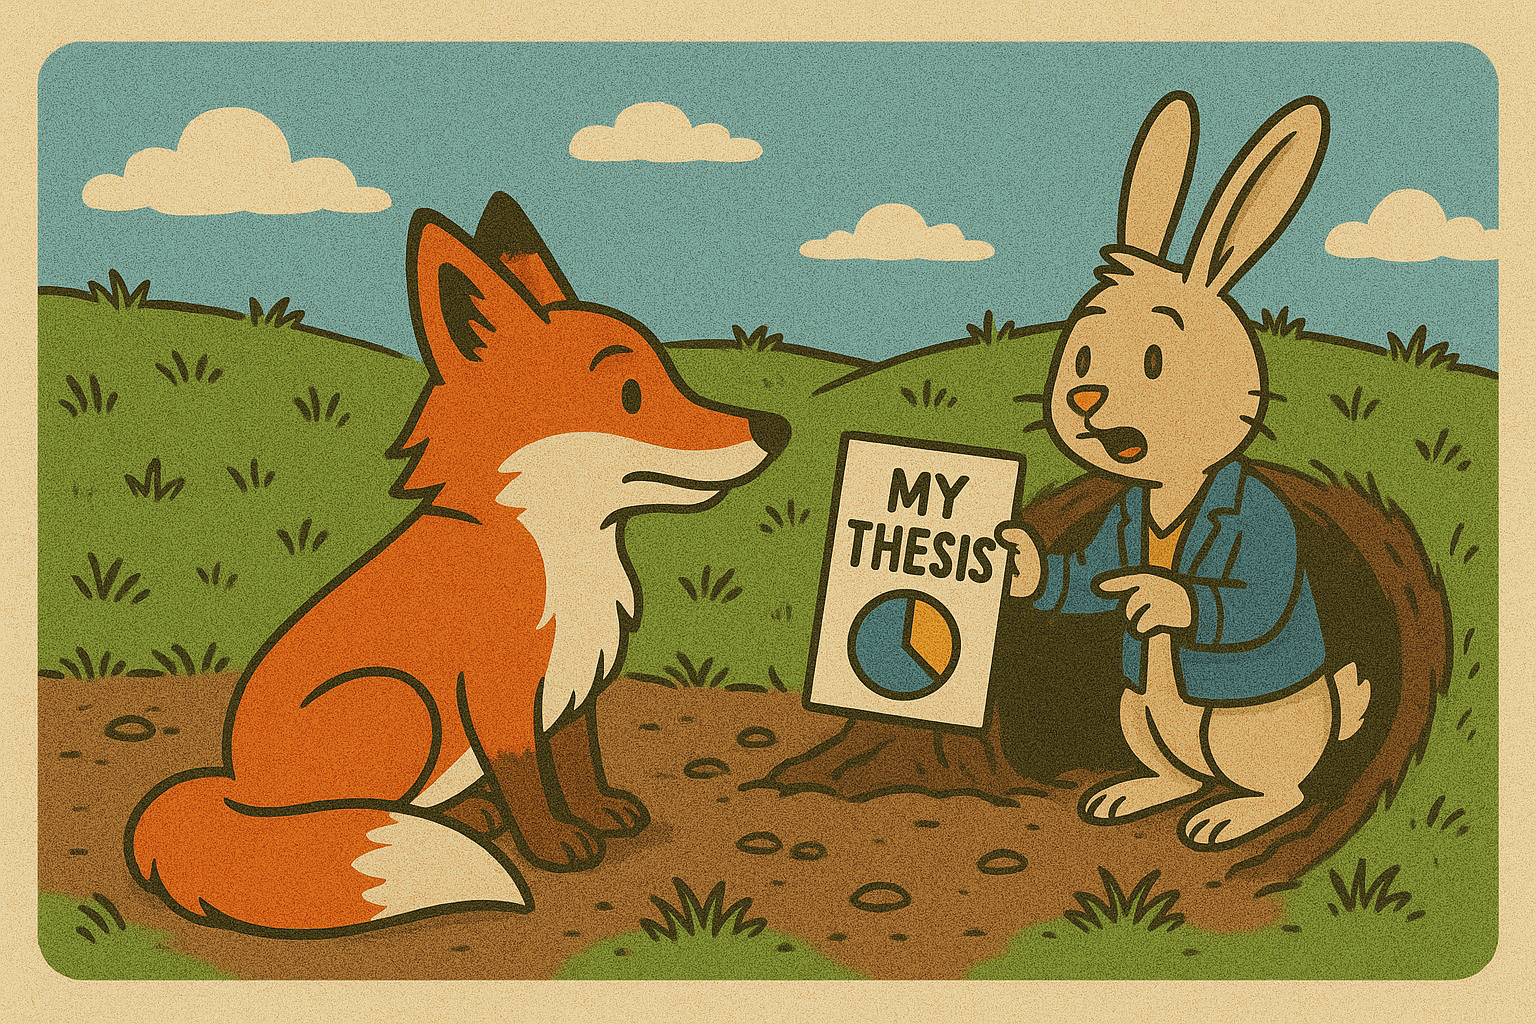
\includegraphics[width=0.5\linewidth]{Images/coelho.png}    
\end{center}
\vspace{0.5cm}


Lembrem que toda piada tem um grau de verdade

\section{O Gênio }

Três sujeitos caminhando lado a lado, na hora do almoço. O orientador, o Bolsista de pós-graduação e o Bolsista de Graduação.

De repente, eles veem uma lâmpada velha, dessas bem antigas, das MIL e UMA Noites. O orientador pega a tal lâmpada e dá uma esfregadinha com a mão...

Logo aparece uma fumaceira e sai um Gênio, daqueles grandes, logo dizendo.... ``Normalmente eu concedo UM desejo, mas já que vocês são três, um para cada um''...

O bolsista de graduação gritou... ``Primeiro eu, primeiro eu !''

--- OK! -- disse o gênio

--- Gênio, quero ir para as Bahamas, ficar por lá com muitas mulheres colocando uvas na minha boca, à beira da piscina do melhor hotel que tiver por lá e sem nenhum tipo de preocupação monetária ou de saúde.

BUUM ! O cara desapareceu.

--- Agora eu! -- gritou o bolsista de pós-graduação

--- Pode falar -- disse o GÊNIO.

--- Seu Gênio, me manda para Honolulu. Quero duas gatas dessas bem gostosas para me acompanhar, ficar fazendo surf o ano inteiro.

BUUM! Lá foi o cara embora para os Mares do Sul.

Então o Gênio falou para o orientador: ``Agora você !''

E este diz:

--- Quero esses dois de volta no laboratório depois do almoço.

Moral da história:

Deixem o orientador sempre falar primeiro.

\section{A Tese do Coelho}

Num dia lindo e ensolarado, o coelho saiu de sua toca com o notebook e pôs-se a trabalhar, bem concentrado. Pouco depois, passou por ali a raposa e viu aquele suculento coelhinho, tão distraído, que chegou a salivar. No entanto, ela ficou intrigada com a atividade do coelho e aproximou-se, curiosa:

--- Coelhinho, o que você está fazendo aí tão concentrado?

--- Estou redigindo a minha tese de doutorado -- disse o coelho sem tirar os olhos do trabalho.

--- Humm .. . e qual é o tema da sua tese?

--- Ah, é uma teoria provando que os coelhos são os verdadeiros predadores naturais de animais como as raposas.

A raposa fica indignada:

--- Ora! Isso é ridículo! Nós é que somos os predadores dos coelhos!

--- Absolutamente! Venha comigo à minha toca que eu mostro a minha prova experimental.

O coelho e a raposa entram na toca. Poucos instantes depois ouvem-se alguns ruídos indecifráveis, alguns poucos grunhidos e depois silêncio. Em seguida o coelho volta, sozinho, e mais uma vez retoma os trabalhos da sua tese, como se nada tivesse acontecido. Meia hora depois passa um lobo. Ao ver o apetitoso coelhinho tão distraído, agradece mentalmente à cadeia alimentar por estar com o seu jantar garantido. No entanto, o lobo também acha muito curioso um coelho trabalhando naquela concentração toda. O lobo então resolve saber do que se trata aquilo tudo, antes de devorar o coelhinho:

--- Olá, jovem coelhinho. O que o faz trabalhar tão arduamente?

--- Minha tese de doutorado, seu lobo. É uma teoria que venho desenvolvendo há algum tempo e que prova que nós, coelhos, somos os grandes predadores naturais de vários animais carnívoros, inclusive dos lobos.

O lobo não se contém e cai na gargalhada com a petulância do coelho.

--- Apetitoso coelhinho! Isto é um despropósito. Nós, os lobos, é que somos os genuínos predadores naturais dos coelhos. Aliás, chega de conversa...

--- Desculpe-me, mas se você quiser eu posso apresentar a minha prova. Você gostaria de me acompanhar à minha toca?

O lobo não consegue acreditar na sua boa sorte. Ambos desaparecem toca adentro. Alguns instantes depois se ouvem uivos desesperados, ruídos de mastigação e ... silêncio. Mais uma vez o coelho retorna sozinho, impassível, e volta ao trabalho de redação da sua tese, como se nada tivesse acontecido... Dentro da toca do coelho vê-se uma enorme pilha de ossos ensanguentados e pelancas de diversas ex-raposas e, ao lado desta, outra pilha ainda maior de ossos e restos mortais daquilo que um dia foram lobos. Ao centro das duas pilhas de ossos, um enorme LEÃO, satisfeito, bem alimentado e sonolento, a palitar os dentes.

MORAL DA HISTORIA:

\begin{itemize}
\item Não importa quão absurdo é o tema de sua tese.
\item Não importa se você não tem o mínimo fundamento científico.
\item Não importa se os seus experimentos nunca cheguem a provar sua teoria.
\item Não importa nem mesmo se suas idéias vão contra o mais óbvio dos conceitos lógicos...
\item o que importa é quem é seu orientador...
\end{itemize}

\section{Ditados}
\begin{itemize}
\item ``Tudo que é simples dá mais trabalho que merece''
\item ``Se é estúpido, mas funciona, então não é tão estúpido assim.''
\item ``Escopo bom é escopo pequeno''
\item ``Metodologia é função do problema e não o contrário''
\item ``Banca boa é banca de amigos''
\item ``Bibliografia tem de incluir tanto clássicos quanto textos recentes''
\item ``Ciência é Marketing,``venda'' sua tese para a banca''
\item ``Cuidado para não misturar autores incompatíveis''
\item ``Planeje seus experimentos antes de colher os dados, senão você pode não ser capaz de analisá-los.''
\item ``Le mieux est l’ennemi du bien'' -- Atribuída a Voltaire
\item ``Perfection is the enemy of progress'' -- Winston Churchill
\item ``Done is better than perfect'' -- frase usada no desenvolvimento ágil, muitas vezes buscando ``O mais simples que funciona''
\item ``All models are wrong, but some are useful''.  --  George E. P. Box
\item ``Be regular and orderly in your life so that you may be violent and original in your work''  --  Flaubert
\item ``Computer Science is no more about computers than astronomy is about telescopes.''  --  Edsger Dijkstra
\item ``Truth is what stands the test of experience.''  --  Albert Einstein
\item ``The more we know, the more we feel our ignorance; the more we feel how much remains unknown'' --  Sir Humphry Davy
\item ``Science may be described as the art of systematic oversimplification.''  --   Karl Popper
\item ``The great tragedy of Science  --     the slaying of a beautiful hypothesis by an ugly fact.''  --   Thomas Henry Huxley
\item ``The story of a theory's failure often strikes readers as sad and unsatisfying. Since science thrives on self-correction, we who practice this most challenging of human arts do not share such a feeling. We may be unhappy if a favored hypothesis loses or chagrined if theories that we proposed prove inadequate. But refutation almost always contains positive lessons that overwhelm disappointment, even when [...] no new and comprehensive theory has yet filled the void.''  --   Stephen Jay Gould (1941-2002),``Bully for Brontosaurus'', The Face of Miranda (1991)
\item ``There must be no barriers for freedom of inquiry. There is no place for dogma in science. The scientist is free, and must be free to ask any question, to doubt any assertion, to seek for any evidence, to correct any errors.'' -- Robert Oppenheimer
\item ``To know that we know what we know, and to know that we do not know what we do not know, that is true knowledge.'' -- Copernicus
\item ``I believe there is no philosophical high-road in science, with epistemological signposts. No, we are in a jungle and find our way by trial and error, building our road behind us as we proceed.'' -- Max Born
\item ``Nothing in this world is to be feared... only understood.'' -- Marie Curie
\item ``The fact that some geniuses were laughed at does not imply that all who are laughed at are geniuses. They laughed at Columbus, they laughed at Fulton, they laughed at the Wright brothers. But they also laughed at Bozo the Clown.'' -- Carl Sagan
\item	“A scientist is happy, not in resting on his attainments but in the steady acquisition of fresh knowledge.'' -- Max Planck
\item ``It doesn't matter how beautiful your theory is, it doesn't matter how smart you are. If it doesn't agree with experiment, it's wrong'' -- Richard Feynman
\item	Crash programs fail because they are based on theory that, with nine women pregnant, you can get a baby a month -- Wernher von Braun.
\item	Early to bed, early to rise, work like hell and advertise -- Wernher von Braun.
\item	One test result is worth one thousand expert opinions -- Wernher von Braun.
\item	Science does not have a moral dimension. It is like a knife. If you give it to a surgeon or a murderer, each will use it differently -- Wernher von Braun.
\item	The universe is hostile only when you do not know its laws. To those who know and obey, the universe is friendly -- Wernher von Braun.
\item	With every new answer unfolded, science has consistently discovered at least three new questions -- Wernher von Braun.
\end{itemize}


Quadrinhos sobre doutorandos podem ser encontrados no site PhdComics.

